\chapter{Figures}

\vspace*{-3in}

\begin{figure}
\vspace{2.4in}
\centering
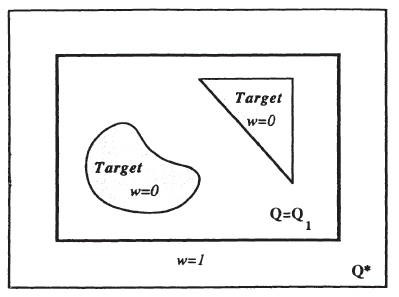
\includegraphics[scale=1]{bvpregions}
\caption{A state space divided into capture,escape, and regions of play \cite{bardi2}}
\label{bvpregions}
\end{figure}
\clearpage
\newpage

\begin{figure}
\vspace{2.4in}
\centering
\begin{subfigure}[b]{0.475\textwidth}
	\centering
	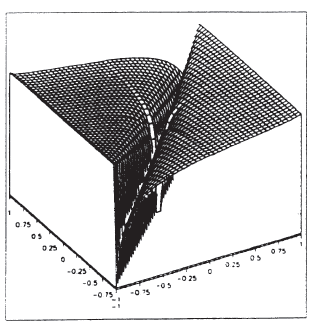
\includegraphics[width=\textwidth]{bvpresult1}
	\caption{Approximate value function when $v_1 = 1$, $v_2 = 1$}
	\label{bvpresult1}
\end{subfigure}
\hfill
\begin{subfigure}[b]{0.475\textwidth}
	\centering
	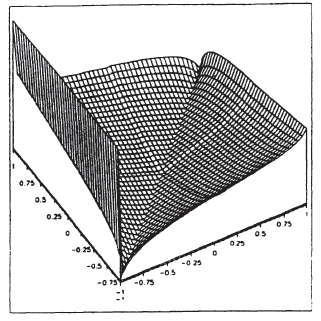
\includegraphics[width=\textwidth]{bvpresult2}
	\caption{Approximate value function when $v_1 = 5$, $v_2 = 1$}
	\label{bvpresult2}
\end{subfigure}
\caption{Results for one-dimensional pursuit-evasion games \cite{bardi2}}
\label{bvpresults}
\end{figure}
\clearpage
\newpage

\begin{figure}
\vspace{2.4in}
\centering
\begin{subfigure}[b]{0.475\textwidth}
	\centering
	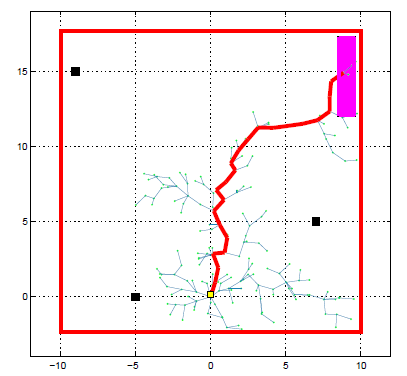
\includegraphics[width=\textwidth]{rrt500}
	\caption{Pursuit-Evasion $\textnormal{RRT}^*$ run for 500 iterations }
	\label{rrt500}
\end{subfigure}
\hfill
\begin{subfigure}[b]{0.475\textwidth}
	\centering
	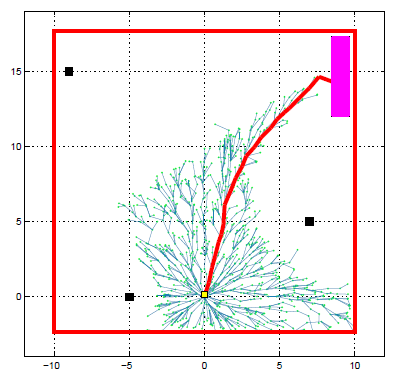
\includegraphics[width=\textwidth]{rrt3000}
	\caption{Pursuit-Evasion $\textnormal{RRT}^*$ run for 3000 iterations}
	\label{rrt3000}
\end{subfigure}
\vskip\baselineskip
\begin{subfigure}[b]{0.475\textwidth}
	\centering
	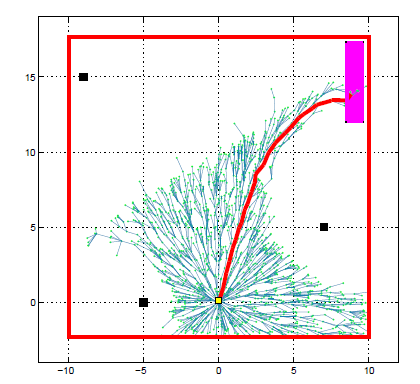
\includegraphics[width=\textwidth]{rrt5000}
	\caption{Pursuit-Evasion $\textnormal{RRT}^*$ run for 5000 iterations}
	\label{rrt5000}
\end{subfigure}
\quad
\begin{subfigure}[b]{0.475\textwidth}
	\centering
	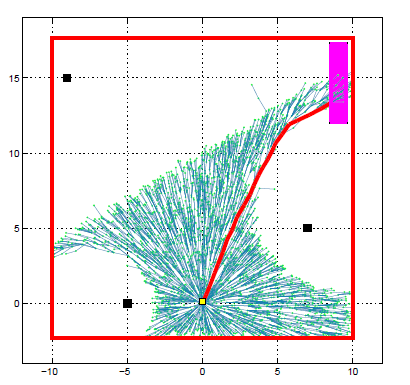
\includegraphics[width=\textwidth]{rrt10000}
	\caption{Pursuit-Evasion $\textnormal{RRT}^*$ run for 10000 iterations}
	\label{rrt10000}
\end{subfigure}
\caption{Pursuit-Evasion $\textnormal{RRT}^*$ \cite{karaman}}
\label{rrtfig}
\end{figure}
\clearpage
\newpage

\begin{figure}
\vspace{2.4in}
\centering
\begin{subfigure}[b]{0.475\textwidth}
	\centering
	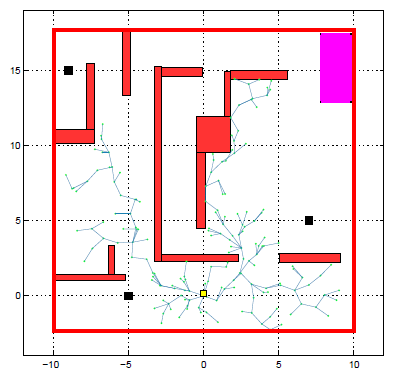
\includegraphics[width=\textwidth]{rrtobs500}
	\caption{Pursuit-Evasion $\textnormal{RRT}^*$ run for 500 iterations}
	\label{rrtobs500}
\end{subfigure}
\hfill
\begin{subfigure}[b]{0.475\textwidth}
	\centering
	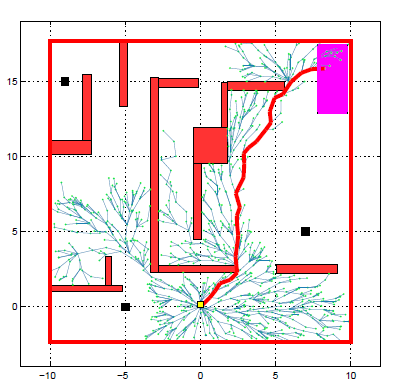
\includegraphics[width=\textwidth]{rrtobs3000}
	\caption{Pursuit-Evasion $\textnormal{RRT}^*$ run for 3000 iterations}
	\label{rrtobs3000}
\end{subfigure}
\vskip\baselineskip
\begin{subfigure}[b]{0.475\textwidth}
	\centering
	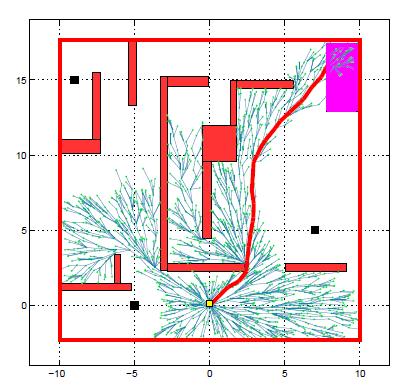
\includegraphics[width=\textwidth]{rrtobs5000}
	\caption{Pursuit-Evasion $\textnormal{RRT}^*$ run for 5000 iterations}
	\label{rrtobs5000}
\end{subfigure}
\quad
\begin{subfigure}[b]{0.475\textwidth}
	\centering
	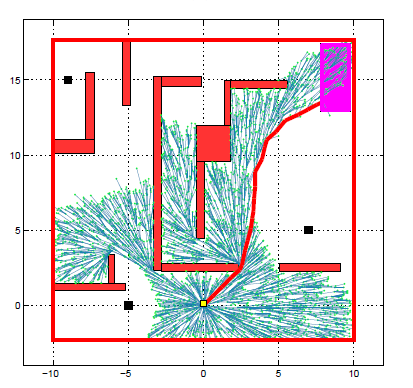
\includegraphics[width=\textwidth]{rrtobs10000}
	\caption{Pursuit-Evasion $\textnormal{RRT}^*$ run for 10000 iterations}
	\label{rrtobs10000}
\end{subfigure}
\caption{Pursuit-Evasion $\textnormal{RRT}^*$ in a field with obstacles\cite{karaman}}
\label{rrtobsfig}
\end{figure}
\clearpage
\newpage

\begin{figure}
\vspace{2.4in}
\centering
\begin{subfigure}[b]{0.475\textwidth}
	\centering
	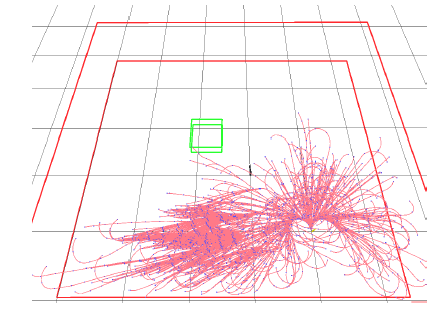
\includegraphics[width=\textwidth]{rrtdubins}
	\caption{Pursuit-Evasion $\textnormal{RRT}^*$ run for 3000 iterations}
	\label{rrtdubins}
\end{subfigure}
\hfill
\begin{subfigure}[b]{0.475\textwidth}
	\centering
	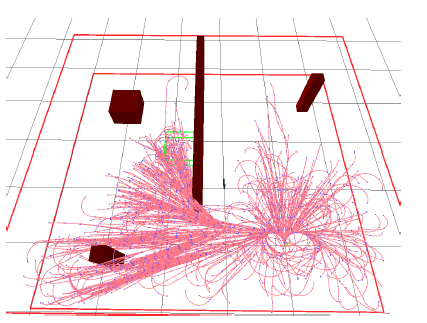
\includegraphics[width=\textwidth]{rrtobsdubins}
	\caption{Pursuit-Evasion $\textnormal{RRT}^*$ run for 3000 iterations in a field with obstacles}
	\label{rrtobsdubins}
\end{subfigure}
\caption{Pursuit-Evasion $\textnormal{RRT}^*$ on a problem with Dubins dynamics \cite{karaman}}
\label{rrtdubinsfig}
\end{figure}
\clearpage
\newpage

\begin{figure}
\vspace{2.4in}
\centering
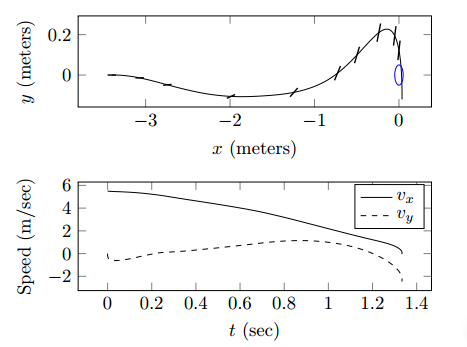
\includegraphics[scale=1]{gorodglide}
\caption{Optimal glide path with vertical and horizontal velocities \cite{gorod}}
\label{gorodglide}
\end{figure}
\clearpage
\newpage

\begin{figure}
\vspace{2.4in}
\centering
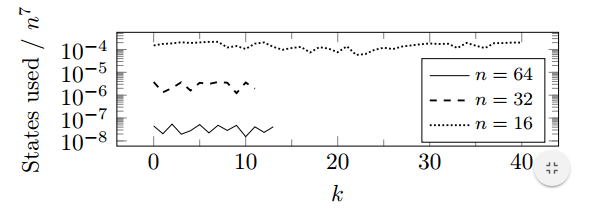
\includegraphics[scale=1]{gorodstates}
\caption{Fraction of states evaluated by TTVI in optimal glide problem \cite{gorod}}
\label{gorodstates}
\end{figure}
\clearpage
\newpage

\begin{figure}
\vspace{2.4in}
\centering
\includegraphics[scale=3]{VIpursplot1}
\caption{Pursuer at (1,1) captures stationary evader at (5,5) after the first Pursuit Value Iteration Run}
\label{VIpursplot1}
\end{figure}
\clearpage
\newpage

\begin{figure}
\vspace{2.4in}
\centering
\includegraphics[scale=3]{VIpursplot2}
\caption{Pursuer at (5,1) captures stationary evader at (5,5) after the first Pursuit Value Iteration Run}
\label{VIpursplot2}
\end{figure}
\clearpage
\newpage

\begin{figure}
\vspace{2.4in}
\centering
\includegraphics[scale=3]{VIpursplot3}
\caption{Pursuer at (9,1) captures stationary evader at (5,5) after the first Pursuit Value Iteration Run}
\label{VIpursplot3}
\end{figure}
\clearpage
\newpage

\begin{figure}
\vspace{2.4in}
\centering
\includegraphics[scale=3]{VIpursplot4}
\caption{Pursuer at (9,5) captures stationary evader at (5,5) after the first Pursuit Value Iteration Run}
\label{VIpursplot4}
\end{figure}
\clearpage
\newpage

\begin{figure}
\vspace{2.4in}
\centering
\includegraphics[scale=3]{VIpursplot5}
\caption{Pursuer at (9,9) captures stationary evader at (5,5) after the first Pursuit Value Iteration Run}
\label{VIpursplot5}
\end{figure}
\clearpage
\newpage

\begin{figure}
\vspace{2.4in}
\centering
\includegraphics[scale=3]{VIpursplot6}
\caption{Pursuer at (5,9) captures stationary evader at (5,5) after the first Pursuit Value Iteration Run}
\label{VIpursplot6}
\end{figure}
\clearpage
\newpage

\begin{figure}
\vspace{2.4in}
\centering
\includegraphics[scale=3]{VIpursplot7}
\caption{Pursuer at (1,9) captures stationary evader at (5,5) after the first Pursuit Value Iteration Run}
\label{VIpursplot7}
\end{figure}
\clearpage
\newpage

\begin{figure}
\vspace{2.4in}
\centering
\includegraphics[scale=3]{VIpursplot8}
\caption{Pursuer at (1,5) captures stationary evader at (5,5) after the first Pursuit Value Iteration Run}
\label{VIpursplot8}
\end{figure}
\clearpage
\newpage

\begin{figure}
\vspace{2.4in}
\centering
\includegraphics[scale=0.25]{VIpursue0}
\caption{State Cost of the Pursuer when the Evader is at (5,5) after one iteration}
\label{VIpursue0}
\end{figure}
\clearpage
\newpage

\begin{figure}
\vspace{2.4in}
\centering
\includegraphics[scale=0.25]{VIpursue10}
\caption{State Cost of the Pursuer when the Evader is at (5,5) after eleven iterations}
\label{VIpursue10}
\end{figure}
\clearpage
\newpage

\begin{figure}
\vspace{2.4in}
\centering
\includegraphics[scale=0.25]{VIpursue98}
\caption{State Cost of the Pursuer when the Evader is at (5,5) after ninety-nine iterations}
\label{VIpursue98}
\end{figure}
\clearpage
\newpage

\begin{figure}
\vspace{2.4in}
\centering
\includegraphics[scale=0.25]{VIpursue99}
\caption{State Cost of the Pursuer when the Evader is at (5,5) after a hundred iterations}
\label{VIpursue99}
\end{figure}
\clearpage
\newpage

\begin{figure}
\vspace{2.4in}
\centering
\includegraphics[scale=3]{VIevadplot1}
\caption{Evader at (5,5) evades stationary pursuer at (1,1) after the first Evade Value Iteration Run}
\label{VIevadplot1}
\end{figure}
\clearpage
\newpage

\begin{figure}
\vspace{2.4in}
\centering
\includegraphics[scale=3]{VIevadplot2}
\caption{Evader at (5,5) evades stationary pursuer at (5,1) after the first Evade Value Iteration Run}
\label{VIevadplot2}
\end{figure}
\clearpage
\newpage

\begin{figure}
\vspace{2.4in}
\centering
\includegraphics[scale=3]{VIevadplot3}
\caption{Evader at (5,5) evades stationary pursuer at (9,1) after the first Evade Value Iteration Run}
\label{VIevadplot3}
\end{figure}
\clearpage
\newpage

\begin{figure}
\vspace{2.4in}
\centering
\includegraphics[scale=3]{VIevadplot4}
\caption{Evader at (5,5) evades stationary pursuer at (9,5) after the first Evade Value Iteration Run}
\label{VIevadplot4}
\end{figure}
\clearpage
\newpage

\begin{figure}
\vspace{2.4in}
\centering
\includegraphics[scale=3]{VIevadplot5}
\caption{Evader at (5,5) evades stationary pursuer at (9,9) after the first Evade Value Iteration Run}
\label{VIevadplot5}
\end{figure}
\clearpage
\newpage

\begin{figure}
\vspace{2.4in}
\centering
\includegraphics[scale=3]{VIevadplot6}
\caption{Evader at (5,5) evades stationary pursuer at (5,9) after the first Evade Value Iteration Run}
\label{VIevadplot6}
\end{figure}
\clearpage
\newpage

\begin{figure}
\vspace{2.4in}
\centering
\includegraphics[scale=3]{VIevadplot7}
\caption{Evader at (5,5) evades stationary pursuer at (1,9) after the first Evade Value Iteration Run}
\label{VIevadplot7}
\end{figure}
\clearpage
\newpage

\begin{figure}
\vspace{2.4in}
\centering
\includegraphics[scale=3]{VIevadplot8}
\caption{Evader at (5,5) evades stationary pursuer at (1,5) after the first Evade Value Iteration Run}
\label{VIevadplot8}
\end{figure}
\clearpage
\newpage

\begin{figure}
\vspace{2.4in}
\centering
\includegraphics[scale=0.25]{VIevade0}
\caption{State Cost of the Evader when the Pursuer is at (1,1) after one iteration}
\label{VIevade0}
\end{figure}
\clearpage
\newpage

\begin{figure}
\vspace{2.4in}
\centering
\includegraphics[scale=0.25]{VIevade10}
\caption{State Cost of the Evader when the Pursuer is at (1,1) after elven iterations}
\label{VIevade10}
\end{figure}
\clearpage
\newpage

\begin{figure}
\vspace{2.4in}
\centering
\includegraphics[scale=0.25]{VIevade98}
\caption{State Cost of the Evader when the Pursuer is at (1,1) after ninety-nine iterations}
\label{VIevade98}
\end{figure}
\clearpage
\newpage

\begin{figure}
\vspace{2.4in}
\centering
\includegraphics[scale=0.25]{VIevade99}
\caption{State Cost of the Evader when the Pursuer is at (1,1) after a hundred iterations}
\label{VIevade99}
\end{figure}
\clearpage
\newpage

\begin{figure}
\vspace{2.4in}
\centering
\includegraphics[scale=3]{VIpursbr1plot1}
\caption{Pursuer at (1,1) captures evader at (5,5) after the second Pursuit Value Iteration Run}
\label{VIpursbr1plot1}
\end{figure}
\clearpage
\newpage

\begin{figure}
\vspace{2.4in}
\centering
\includegraphics[scale=3]{VIpursbr1plot2}
\caption{Pursuer at (5,1) captures evader at (5,5) after the second Pursuit Value Iteration Run}
\label{VIpursbr1plot2}
\end{figure}
\clearpage
\newpage

\begin{figure}
\vspace{2.4in}
\centering
\includegraphics[scale=3]{VIpursbr1plot3}
\caption{Pursuer at (9,1) captures evader at (5,5) after the second Pursuit Value Iteration Run}
\label{VIpursbr1plot3}
\end{figure}
\clearpage
\newpage

\begin{figure}
\vspace{2.4in}
\centering
\includegraphics[scale=3]{VIpursbr1plot4}
\caption{Pursuer at (9,5) captures evader at (5,5) after the second Pursuit Value Iteration Run}
\label{VIpursbr1plot4}
\end{figure}
\clearpage
\newpage

\begin{figure}
\vspace{2.4in}
\centering
\includegraphics[scale=3]{VIpursbr1plot5}
\caption{Pursuer at (9,9) captures evader at (5,5) after the second Pursuit Value Iteration Run}
\label{VIpursbr1plot5}
\end{figure}
\clearpage
\newpage

\begin{figure}
\vspace{2.4in}
\centering
\includegraphics[scale=3]{VIpursbr1plot6}
\caption{Pursuer at (5,9) captures evader at (5,5) after the second Pursuit Value Iteration Run}
\label{VIpursbr1plot6}
\end{figure}
\clearpage
\newpage

\begin{figure}
\vspace{2.4in}
\centering
\includegraphics[scale=3]{VIpursbr1plot7}
\caption{Pursuer at (1,9) captures evader at (5,5) after the second Pursuit Value Iteration Run}
\label{VIpursbr1plot7}
\end{figure}
\clearpage
\newpage

\begin{figure}
\vspace{2.4in}
\centering
\includegraphics[scale=3]{VIpursbr1plot8}
\caption{Pursuer at (1,5) captures evader at (5,5) after the second Pursuit Value Iteration Run}
\label{VIpursbr1plot8}
\end{figure}
\clearpage
\newpage

\begin{figure}
\vspace{2.4in}
\centering
\includegraphics[scale=0.25]{VIpursue1br0}
\caption{State Cost of the Pursuer when the Evader is at (5,5) after one iteration}
\label{VIpursue1br0}
\end{figure}
\clearpage
\newpage

\begin{figure}
\vspace{2.4in}
\centering
\includegraphics[scale=0.25]{VIpursue1br10}
\caption{State Cost of the Pursuer when the Evader is at (5,5) after eleven iterations}
\label{VIpursue1br10}
\end{figure}
\clearpage
\newpage

\begin{figure}
\vspace{2.4in}
\centering
\includegraphics[scale=0.25]{VIpursue1br98}
\caption{State Cost of the Pursuer when the Evader is at (5,5) after ninety-nine iterations}
\label{VIpursue1br98}
\end{figure}
\clearpage
\newpage

\begin{figure}
\vspace{2.4in}
\centering
\includegraphics[scale=0.25]{VIpursue1br99}
\caption{State Cost of the Pursuer when the Evader is at (5,5) after a hundred iterations}
\label{VIpursue1br99}
\end{figure}
\clearpage
\newpage

\begin{figure}
\vspace{2.4in}
\centering
\includegraphics[scale=3]{VIevadbrplot1}
\caption{Pursuer at (1,1) captures evader at (5,5) after the second Evade Value Iteration Run}
\label{VIevadbrplot1}
\end{figure}
\clearpage
\newpage

\begin{figure}
\vspace{2.4in}
\centering
\includegraphics[scale=3]{VIevadbrplot2}
\caption{Pursuer at (5,1) captures evader at (5,5) after the second Evade Value Iteration Run}
\label{VIevadbrplot2}
\end{figure}
\clearpage
\newpage

\begin{figure}
\vspace{2.4in}
\centering
\includegraphics[scale=3]{VIevadbrplot3}
\caption{Pursuer at (9,1) captures evader at (5,5) after the second Evade Value Iteration Run}
\label{VIevadbrplot3}
\end{figure}
\clearpage
\newpage

\begin{figure}
\vspace{2.4in}
\centering
\includegraphics[scale=3]{VIevadbrplot4}
\caption{Pursuer at (9,5) captures evader at (5,5) after the second Evade Value Iteration Run}
\label{VIevadbrplot4}
\end{figure}
\clearpage
\newpage

\begin{figure}
\vspace{2.4in}
\centering
\includegraphics[scale=3]{VIevadbrplot5}
\caption{Pursuer at (9,9) captures evader at (5,5) after the second Evade Value Iteration Run}
\label{VIevadbrplot5}
\end{figure}
\clearpage
\newpage

\begin{figure}
\vspace{2.4in}
\centering
\includegraphics[scale=3]{VIevadbrplot6}
\caption{Pursuer at (5,9) captures evader at (5,5) after the second Evade Value Iteration Run}
\label{VIevadbrplot6}
\end{figure}
\clearpage
\newpage

\begin{figure}
\vspace{2.4in}
\centering
\includegraphics[scale=3]{VIevadbrplot7}
\caption{Pursuer at (1,9) captures evader at (5,5) after the second Evade Value Iteration Run}
\label{VIevadbrplot7}
\end{figure}
\clearpage
\newpage

\begin{figure}
\vspace{2.4in}
\centering
\includegraphics[scale=3]{VIevadbrplot8}
\caption{Pursuer at (1,5) captures evader at (5,5) after the second Evade Value Iteration Run}
\label{VIevadbrplot8}
\end{figure}
\clearpage
\newpage

\begin{figure}
\vspace{2.4in}
\centering
\includegraphics[scale=0.25]{VIevadebr0}
\caption{State Cost of the Evader when the Pursuer is at (1,1) after one iteration}
\label{VIevadebr0}
\end{figure}
\clearpage
\newpage

\begin{figure}
\vspace{2.4in}
\centering
\includegraphics[scale=0.25]{VIevadebr10}
\caption{State Cost of the Evader when the Pursuer is at (1,1) after elven iterations}
\label{VIevadebr10}
\end{figure}
\clearpage
\newpage

\begin{figure}
\vspace{2.4in}
\centering
\includegraphics[scale=0.25]{VIevadebr98}
\caption{State Cost of the Evader when the Pursuer is at (1,1) after ninety-nine iterations}
\label{VIevadebr98}
\end{figure}
\clearpage
\newpage

\begin{figure}
\vspace{2.4in}
\centering
\includegraphics[scale=0.25]{VIevadebr99}
\caption{State Cost of the Evader when the Pursuer is at (1,1) after a hundred iterations}
\label{VIevadebr99}
\end{figure}
\clearpage
\newpage

\begin{figure}
\vspace{2.4in}
\centering
\includegraphics[scale=3]{VIpursbr2plot1}
\caption{Pursuer at (1,1) captures evader at (5,5) after the third Pursuit Value Iteration Run}
\label{VIpursbr2plot1}
\end{figure}
\clearpage
\newpage

\begin{figure}
\vspace{2.4in}
\centering
\includegraphics[scale=3]{VIpursbr2plot2}
\caption{Pursuer at (5,1) captures evader at (5,5) after the third Pursuit Value Iteration Run}
\label{VIpursbr2plot2}
\end{figure}
\clearpage
\newpage

\begin{figure}
\vspace{2.4in}
\centering
\includegraphics[scale=3]{VIpursbr2plot3}
\caption{Pursuer at (9,1) captures evader at (5,5) after the third Pursuit Value Iteration Run}
\label{VIpursbr2plot3}
\end{figure}
\clearpage
\newpage

\begin{figure}
\vspace{2.4in}
\centering
\includegraphics[scale=3]{VIpursbr2plot4}
\caption{Pursuer at (9,5) captures evader at (5,5) after the third Pursuit Value Iteration Run}
\label{VIpursbr2plot4}
\end{figure}
\clearpage
\newpage

\begin{figure}
\vspace{2.4in}
\centering
\includegraphics[scale=3]{VIpursbr2plot5}
\caption{Pursuer at (9,9) captures evader at (5,5) after the third Pursuit Value Iteration Run}
\label{VIpursbr2plot5}
\end{figure}
\clearpage
\newpage

\begin{figure}
\vspace{2.4in}
\centering
\includegraphics[scale=3]{VIpursbr2plot6}
\caption{Pursuer at (5,9) captures evader at (5,5) after the third Pursuit Value Iteration Run}
\label{VIpursbr2plot6}
\end{figure}
\clearpage
\newpage

\begin{figure}
\vspace{2.4in}
\centering
\includegraphics[scale=3]{VIpursbr2plot7}
\caption{Pursuer at (1,9) captures evader at (5,5) after the third Pursuit Value Iteration Run}
\label{VIpursbr2plot7}
\end{figure}
\clearpage
\newpage

\begin{figure}
\vspace{2.4in}
\centering
\includegraphics[scale=3]{VIpursbr2plot8}
\caption{Pursuer at (1,5) captures evader at (5,5) after the third Pursuit Value Iteration Run}
\label{VIpursbr2plot8}
\end{figure}
\clearpage
\newpage

\begin{figure}
\vspace{2.4in}
\centering
\includegraphics[scale=0.25]{VIpursue2br0}
\caption{State Cost of the Pursuer when the Evader is at (5,5) after one iteration}
\label{VIpursue2br0}
\end{figure}
\clearpage
\newpage

\begin{figure}
\vspace{2.4in}
\centering
\includegraphics[scale=0.25]{VIpursue2br99}
\caption{State Cost of the Pursuer when the Evader is at (5,5) after a hundred iterations}
\label{VIpursue2br99}
\end{figure}
\clearpage
\newpage

\begin{figure}
\vspace{2.4in}
\centering
\includegraphics[scale=3]{4DTradPurs0diffNormplot}
\caption{Change in Norm of Pursuer State Value for each iteration of traditional VI}
\label{4DTradPurs0diffNormplot}
\end{figure}
\clearpage
\newpage

\begin{figure}
\vspace{2.4in}
\centering
\includegraphics[scale=3]{4DTradPurs0normplot}
\caption{Norm of Pursuer State Value for each iteration of traditional VI}
\label{4DTradPurs0normplot}
\end{figure}
\clearpage
\newpage

\begin{figure}
\vspace{2.4in}
\centering
\includegraphics[scale=3]{4DTradEvad0diffNormplot}
\caption{Change in Norm of Evader State Value for each iteration of traditional VI}
\label{4DTradEvad0diffNormplot}
\end{figure}
\clearpage
\newpage

\begin{figure}
\vspace{2.4in}
\centering
\includegraphics[scale=3]{4DTradEvad0normplot}
\caption{Norm of Evader State Value for each iteration of traditional VI}
\label{4DTradEvad0normplot}
\end{figure}
\clearpage
\newpage

\begin{figure}
\vspace{2.4in}
\centering
\includegraphics[scale=3]{4DTradPurs1diffNormplot}
\caption{Change in Norm of Pursuer State Value for each iteration of traditional VI}
\label{4DTradPurs1diffNormplot}
\end{figure}
\clearpage
\newpage

\begin{figure}
\vspace{2.4in}
\centering
\includegraphics[scale=3]{4DTradPurs1normplot}
\caption{Norm of Pursuer State Value for each iteration of traditional VI}
\label{4DTradPurs1normplot}
\end{figure}
\clearpage
\newpage

\begin{figure}
\vspace{2.4in}
\centering
\includegraphics[scale=3]{4DTradPurspurscolorplot}
\caption{Pursuer State Value when Evader is at (5,5)}
\label{4DTradPurspurscolorplot}
\end{figure}
\clearpage
\newpage

\begin{figure}
\vspace{2.4in}
\centering
\includegraphics[scale=3]{4DTradEvad1diffNormplot}
\caption{Change in Norm of Evader State Value for each iteration of traditional VI}
\label{4DTradEvad1diffNormplot}
\end{figure}
\clearpage
\newpage

\begin{figure}
\vspace{2.4in}
\centering
\includegraphics[scale=3]{4DTradEvad1normplot}
\caption{Norm of Evader State Value for each iteration of traditional VI}
\label{4DTradEvad1normplot}
\end{figure}
\clearpage
\newpage

\begin{figure}
\vspace{2.4in}
\centering
\includegraphics[scale=3]{4DTradEvadevadcolorplot}
\caption{Evader State Value when Pursuer is at (1,1)}
\label{4DTradEvadevadcolorplot}
\end{figure}
\clearpage
\newpage

\begin{figure}
\vspace{2.4in}
\centering
\includegraphics[scale=3]{4DTradEvadmovieplot0}
\caption{Start of pursuit-Evasion game with pursuer starting at (1,1) and the evader starting at (5,5)}
\label{4DTradEvadmovieplot0}
\end{figure}
\clearpage
\newpage

\begin{figure}
\vspace{2.4in}
\centering
\includegraphics[scale=3]{4DTradEvadmovieplot1}
\caption{Pursuit-Evasion game with pursuer starting at (1,1) and the evader starting at (5,5) after 1 second}
\label{4DTradEvadmovieplot1}
\end{figure}
\clearpage
\newpage

\begin{figure}
\vspace{2.4in}
\centering
\includegraphics[scale=3]{4DTradEvadmovieplot2}
\caption{Pursuit-Evasion game with pursuer starting at (1,1) and the evader starting at (5,5) after 2 second}
\label{4DTradEvadmovieplot2}
\end{figure}
\clearpage
\newpage

\begin{figure}
\vspace{2.4in}
\centering
\includegraphics[scale=3]{4DTradEvadmovieplot3}
\caption{Pursuit-Evasion game with pursuer starting at (1,1) and the evader starting at (5,5) after 3 second}
\label{4DTradEvadmovieplot3}
\end{figure}
\clearpage
\newpage

\begin{figure}
\vspace{2.4in}
\centering
\includegraphics[scale=3]{4DTradEvadmovieplot4}
\caption{Pursuit-Evasion game with pursuer starting at (1,1) and the evader starting at (5,5) after 4 second}
\label{4DTradEvadmovieplot4}
\end{figure}
\clearpage
\newpage

\begin{figure}
\vspace{2.4in}
\centering
\includegraphics[scale=3]{4DTradEvadmovieplot5}
\caption{Pursuit-Evasion game with pursuer starting at (1,1) and the evader starting at (5,5) after 5 second}
\label{4DTradEvadmovieplot5}
\end{figure}
\clearpage
\newpage

\begin{figure}
\vspace{2.4in}
\centering
\includegraphics[scale=3]{4DTradEvadmovieplot6}
\caption{Pursuit-Evasion game with pursuer starting at (1,1) and the evader starting at (5,5) after 6 second}
\label{4DTradEvadmovieplot6}
\end{figure}
\clearpage
\newpage

\begin{figure}
\vspace{2.4in}
\centering
\includegraphics[scale=3]{4DTradEvadmovieplot7}
\caption{Pursuit-Evasion game with pursuer starting at (1,1) and the evader starting at (5,5) after 7 second}
\label{4DTradEvadmovieplot7}
\end{figure}
\clearpage
\newpage

\begin{figure}
\vspace{2.4in}
\centering
\includegraphics[scale=3]{4DTradEvadmovieplot8}
\caption{Pursuit-Evasion game with pursuer starting at (1,1) and the evader starting at (5,5) after 8 second}
\label{4DTradEvadmovieplot8}
\end{figure}
\clearpage
\newpage

\begin{figure}
\vspace{2.4in}
\centering
\includegraphics[scale=3]{4DTradEvadmovieplot9}
\caption{Pursuit-Evasion game with pursuer starting at (1,1) and the evader starting at (5,5) after 9 second}
\label{4DTradEvadmovieplot9}
\end{figure}
\clearpage
\newpage

\begin{figure}
\vspace{2.4in}
\centering
\includegraphics[scale=3]{4DTradEvadphaseplot}
\caption{Pursuit-Evasion game with pursuer starting at (1,1) and the evader starting at (5,5) at one second intervals}
\label{4DTradEvadphaseplot}
\end{figure}
\clearpage
\newpage

\begin{figure}
\vspace{2.4in}
\centering
\includegraphics[scale=3]{4DTradEvadrelplot}
\caption{Relative position between pursuer starting at (1,1) and the evader starting at (5,5)}
\label{4DTradEvadrelplot}
\end{figure}
\clearpage
\newpage

\begin{figure}
\vspace{2.4in}
\centering
\includegraphics[scale=3]{4DCompPurs0diffNormplot}
\caption{Change in Norm of Pursuer State Value for each iteration of traditional VI}
\label{4DCompPurs0diffNormplot}
\end{figure}
\clearpage
\newpage

\begin{figure}
\vspace{2.4in}
\centering
\includegraphics[scale=3]{4DCompPurs0normplot}
\caption{Norm of Pursuer State Value for each iteration of traditional VI}
\label{4DCompPurs0normplot}
\end{figure}
\clearpage
\newpage

\begin{figure}
\vspace{2.4in}
\centering
\includegraphics[scale=3]{4DCompEvad0diffNormplot}
\caption{Change in Norm of Evader State Value for each iteration of traditional VI}
\label{4DCompEvad0diffNormplot}
\end{figure}
\clearpage
\newpage

\begin{figure}
\vspace{2.4in}
\centering
\includegraphics[scale=3]{4DCompEvad0normplot}
\caption{Norm of Evader State Value for each iteration of traditional VI}
\label{4DCompEvad0normplot}
\end{figure}
\clearpage
\newpage

\begin{figure}
\vspace{2.4in}
\centering
\includegraphics[scale=3]{4DCompPurs1diffNormplot}
\caption{Change in Norm of Pursuer State Value for each iteration of traditional VI}
\label{4DCompPurs1diffNormplot}
\end{figure}
\clearpage
\newpage

\begin{figure}
\vspace{2.4in}
\centering
\includegraphics[scale=3]{4DCompPurs1normplot}
\caption{Norm of Pursuer State Value for each iteration of traditional VI}
\label{4DCompPurs1normplot}
\end{figure}
\clearpage
\newpage

\begin{figure}
\vspace{2.4in}
\centering
\includegraphics[scale=3]{4DCompPurspurscolorplot}
\caption{Pursuer State Value when Evader is at (5,5)}
\label{4DCompPurspurscolorplot}
\end{figure}
\clearpage
\newpage

\begin{figure}
\vspace{2.4in}
\centering
\includegraphics[scale=3]{4DCompEvad1diffNormplot}
\caption{Change in Norm of Evader State Value for each iteration of traditional VI}
\label{4DCompEvad1diffNormplot}
\end{figure}
\clearpage
\newpage

\begin{figure}
\vspace{2.4in}
\centering
\includegraphics[scale=3]{4DCompEvad1normplot}
\caption{Norm of Evader State Value for each iteration of traditional VI}
\label{4DCompEvad1normplot}
\end{figure}
\clearpage
\newpage

\begin{figure}
\vspace{2.4in}
\centering
\includegraphics[scale=3]{4DCompEvadevadcolorplot}
\caption{Evader State Value when Pursuer is at (1,1)}
\label{4DCompEvadevadcolorplot}
\end{figure}
\clearpage
\newpage

\begin{figure}
\vspace{2.4in}
\centering
\includegraphics[scale=3]{4DCompEvadmovieplot0}
\caption{Start of pursuit-Evasion game with pursuer starting at (1,1) and the evader starting at (5,5)}
\label{4DCompEvadmovieplot0}
\end{figure}
\clearpage
\newpage

\begin{figure}
\vspace{2.4in}
\centering
\includegraphics[scale=3]{4DCompEvadmovieplot1}
\caption{Pursuit-Evasion game with pursuer starting at (1,1) and the evader starting at (5,5) after 1 second}
\label{4DCompEvadmovieplot1}
\end{figure}
\clearpage
\newpage

\begin{figure}
\vspace{2.4in}
\centering
\includegraphics[scale=3]{4DCompEvadmovieplot2}
\caption{Pursuit-Evasion game with pursuer starting at (1,1) and the evader starting at (5,5) after 2 second}
\label{4DCompEvadmovieplot2}
\end{figure}
\clearpage
\newpage

\begin{figure}
\vspace{2.4in}
\centering
\includegraphics[scale=3]{4DCompEvadmovieplot3}
\caption{Pursuit-Evasion game with pursuer starting at (1,1) and the evader starting at (5,5) after 3 second}
\label{4DCompEvadmovieplot3}
\end{figure}
\clearpage
\newpage

\begin{figure}
\vspace{2.4in}
\centering
\includegraphics[scale=3]{4DCompEvadmovieplot4}
\caption{Pursuit-Evasion game with pursuer starting at (1,1) and the evader starting at (5,5) after 4 second}
\label{4DCompEvadmovieplot4}
\end{figure}
\clearpage
\newpage

\begin{figure}
\vspace{2.4in}
\centering
\includegraphics[scale=3]{4DCompEvadmovieplot5}
\caption{Pursuit-Evasion game with pursuer starting at (1,1) and the evader starting at (5,5) after 5 second}
\label{4DCompEvadmovieplot5}
\end{figure}
\clearpage
\newpage

\begin{figure}
\vspace{2.4in}
\centering
\includegraphics[scale=3]{4DCompEvadmovieplot6}
\caption{Pursuit-Evasion game with pursuer starting at (1,1) and the evader starting at (5,5) after 6 second}
\label{4DCompEvadmovieplot6}
\end{figure}
\clearpage
\newpage

\begin{figure}
\vspace{2.4in}
\centering
\includegraphics[scale=3]{4DCompEvadmovieplot7}
\caption{Pursuit-Evasion game with pursuer starting at (1,1) and the evader starting at (5,5) after 7 second}
\label{4DCompEvadmovieplot7}
\end{figure}
\clearpage
\newpage

\begin{figure}
\vspace{2.4in}
\centering
\includegraphics[scale=3]{4DCompEvadmovieplot8}
\caption{Pursuit-Evasion game with pursuer starting at (1,1) and the evader starting at (5,5) after 8 second}
\label{4DCompEvadmovieplot8}
\end{figure}
\clearpage
\newpage

\begin{figure}
\vspace{2.4in}
\centering
\includegraphics[scale=3]{4DCompEvadmovieplot9}
\caption{Pursuit-Evasion game with pursuer starting at (1,1) and the evader starting at (5,5) after 9 second}
\label{4DCompEvadmovieplot9}
\end{figure}
\clearpage
\newpage

\begin{figure}
\vspace{2.4in}
\centering
\includegraphics[scale=3]{4DCompEvadphaseplot}
\caption{Pursuit-Evasion game with pursuer starting at (1,1) and the evader starting at (5,5) at one second intervals}
\label{4DCompEvadphaseplot}
\end{figure}
\clearpage
\newpage

\begin{figure}
\vspace{2.4in}
\centering
\includegraphics[scale=3]{4DCompEvadrelplot}
\caption{Relative position between pursuer starting at (1,1) and the evader starting at (5,5)}
\label{4DCompEvadrelplot}
\end{figure}
\clearpage
\newpage

\begin{figure}
\vspace{2.4in}
\centering
\includegraphics[scale=3]{TTVIpursplot1}
\caption{Pursuer at (1,1) captures stationary evader at (5,5) after the first Pursuit Value Iteration Run}
\label{TTVIpursplot1}
\end{figure}
\clearpage
\newpage

\begin{figure}
\vspace{2.4in}
\centering
\includegraphics[scale=3]{TTVIpursplot2}
\caption{Pursuer at (5,1) captures stationary evader at (5,5) after the first Pursuit Value Iteration Run}
\label{TTVIpursplot2}
\end{figure}
\clearpage
\newpage

\begin{figure}
\vspace{2.4in}
\centering
\includegraphics[scale=3]{TTVIpursplot3}
\caption{Pursuer at (9,1) captures stationary evader at (5,5) after the first Pursuit Value Iteration Run}
\label{TTVIpursplot3}
\end{figure}
\clearpage
\newpage

\begin{figure}
\vspace{2.4in}
\centering
\includegraphics[scale=3]{TTVIpursplot4}
\caption{Pursuer at (9,5) captures stationary evader at (5,5) after the first Pursuit Value Iteration Run}
\label{TTVIpursplot4}
\end{figure}
\clearpage
\newpage

\begin{figure}
\vspace{2.4in}
\centering
\includegraphics[scale=3]{TTVIpursplot5}
\caption{Pursuer at (9,9) captures stationary evader at (5,5) after the first Pursuit Value Iteration Run}
\label{TTVIpursplot5}
\end{figure}
\clearpage
\newpage

\begin{figure}
\vspace{2.4in}
\centering
\includegraphics[scale=3]{TTVIpursplot6}
\caption{Pursuer at (5,9) captures stationary evader at (5,5) after the first Pursuit Value Iteration Run}
\label{TTVIpursplot6}
\end{figure}
\clearpage
\newpage

\begin{figure}
\vspace{2.4in}
\centering
\includegraphics[scale=3]{TTVIpursplot7}
\caption{Pursuer at (1,9) captures stationary evader at (5,5) after the first Pursuit Value Iteration Run}
\label{TTVIpursplot7}
\end{figure}
\clearpage
\newpage

\begin{figure}
\vspace{2.4in}
\centering
\includegraphics[scale=3]{TTVIpursplot8}
\caption{Pursuer at (1,5) captures stationary evader at (5,5) after the first Pursuit Value Iteration Run}
\label{TTVIpursplot8}
\end{figure}
\clearpage
\newpage

\begin{figure}
\vspace{2.4in}
\centering
\includegraphics[scale=0.25]{TTVIpursue0}
\caption{State Cost of the Pursuer when the Evader is at (5,5) after one iteration}
\label{TTVIpursue0}
\end{figure}
\clearpage
\newpage

\begin{figure}
\vspace{2.4in}
\centering
\includegraphics[scale=0.25]{TTVIpursue10}
\caption{State Cost of the Pursuer when the Evader is at (5,5) after eleven iterations}
\label{TTVIpursue10}
\end{figure}
\clearpage
\newpage

\begin{figure}
\vspace{2.4in}
\centering
\includegraphics[scale=0.25]{TTVIpursue98}
\caption{State Cost of the Pursuer when the Evader is at (5,5) after ninety-nine iterations}
\label{TTVIpursue98}
\end{figure}
\clearpage
\newpage

\begin{figure}
\vspace{2.4in}
\centering
\includegraphics[scale=0.25]{TTVIpursue99}
\caption{State Cost of the Pursuer when the Evader is at (5,5) after a hundred iterations}
\label{TTVIpursue99}
\end{figure}
\clearpage
\newpage

\begin{figure}
\vspace{2.4in}
\centering
\includegraphics[scale=3]{TTVIevadplot1}
\caption{Evader at (5,5) evades stationary pursuer at (1,1) after the first Evade Value Iteration Run}
\label{TTVIevadplot1}
\end{figure}
\clearpage
\newpage

\begin{figure}
\vspace{2.4in}
\centering
\includegraphics[scale=3]{TTVIevadplot2}
\caption{Evader at (5,5) evades stationary pursuer at (5,1) after the first Evade Value Iteration Run}
\label{TTVIevadplot2}
\end{figure}
\clearpage
\newpage

\begin{figure}
\vspace{2.4in}
\centering
\includegraphics[scale=3]{TTVIevadplot3}
\caption{Evader at (5,5) evades stationary pursuer at (9,1) after the first Evade Value Iteration Run}
\label{TTVIevadplot3}
\end{figure}
\clearpage
\newpage

\begin{figure}
\vspace{2.4in}
\centering
\includegraphics[scale=3]{TTVIevadplot4}
\caption{Evader at (5,5) evades stationary pursuer at (9,5) after the first Evade Value Iteration Run}
\label{TTVIevadplot4}
\end{figure}
\clearpage
\newpage

\begin{figure}
\vspace{2.4in}
\centering
\includegraphics[scale=3]{TTVIevadplot5}
\caption{Evader at (5,5) evades stationary pursuer at (9,9) after the first Evade Value Iteration Run}
\label{TTVIevadplot5}
\end{figure}
\clearpage
\newpage

\begin{figure}
\vspace{2.4in}
\centering
\includegraphics[scale=3]{TTVIevadplot6}
\caption{Evader at (5,5) evades stationary pursuer at (5,9) after the first Evade Value Iteration Run}
\label{TTVIevadplot6}
\end{figure}
\clearpage
\newpage

\begin{figure}
\vspace{2.4in}
\centering
\includegraphics[scale=3]{TTVIevadplot7}
\caption{Evader at (5,5) evades stationary pursuer at (1,9) after the first Evade Value Iteration Run}
\label{TTVIevadplot7}
\end{figure}
\clearpage
\newpage

\begin{figure}
\vspace{2.4in}
\centering
\includegraphics[scale=3]{TTVIevadplot8}
\caption{Evader at (5,5) evades stationary pursuer at (1,5) after the first Evade Value Iteration Run}
\label{TTVIevadplot8}
\end{figure}
\clearpage
\newpage

\begin{figure}
\vspace{2.4in}
\centering
\includegraphics[scale=0.25]{TTVIevade0}
\caption{State Cost of the Evader when the Pursuer is at (1,1) after one iteration}
\label{TTVIevade0}
\end{figure}
\clearpage
\newpage

\begin{figure}
\vspace{2.4in}
\centering
\includegraphics[scale=0.25]{TTVIevade10}
\caption{State Cost of the Evader when the Pursuer is at (1,1) after elven iterations}
\label{TTVIevade10}
\end{figure}
\clearpage
\newpage

\begin{figure}
\vspace{2.4in}
\centering
\includegraphics[scale=0.25]{TTVIevade98}
\caption{State Cost of the Evader when the Pursuer is at (1,1) after ninety-nine iterations}
\label{TTVIevade98}
\end{figure}
\clearpage
\newpage

\begin{figure}
\vspace{2.4in}
\centering
\includegraphics[scale=0.25]{TTVIevade99}
\caption{State Cost of the Evader when the Pursuer is at (1,1) after a hundred iterations}
\label{TTVIevade99}
\end{figure}
\clearpage
\newpage

\begin{figure}
\vspace{2.4in}
\centering
\includegraphics[scale=3]{TTVIpursbr1plot1}
\caption{Pursuer at (1,1) captures evader at (5,5) after the second Pursuit Value Iteration Run}
\label{TTVIpursbr1plot1}
\end{figure}
\clearpage
\newpage

\begin{figure}
\vspace{2.4in}
\centering
\includegraphics[scale=3]{TTVIpursbr1plot2}
\caption{Pursuer at (5,1) captures evader at (5,5) after the second Pursuit Value Iteration Run}
\label{TTVIpursbr1plot2}
\end{figure}
\clearpage
\newpage

\begin{figure}
\vspace{2.4in}
\centering
\includegraphics[scale=3]{TTVIpursbr1plot3}
\caption{Pursuer at (9,1) captures evader at (5,5) after the second Pursuit Value Iteration Run}
\label{TTVIpursbr1plot3}
\end{figure}
\clearpage
\newpage

\begin{figure}
\vspace{2.4in}
\centering
\includegraphics[scale=3]{TTVIpursbr1plot4}
\caption{Pursuer at (9,5) captures evader at (5,5) after the second Pursuit Value Iteration Run}
\label{TTVIpursbr1plot4}
\end{figure}
\clearpage
\newpage

\begin{figure}
\vspace{2.4in}
\centering
\includegraphics[scale=3]{TTVIpursbr1plot5}
\caption{Pursuer at (9,9) captures evader at (5,5) after the second Pursuit Value Iteration Run}
\label{TTVIpursbr1plot5}
\end{figure}
\clearpage
\newpage

\begin{figure}
\vspace{2.4in}
\centering
\includegraphics[scale=3]{TTVIpursbr1plot6}
\caption{Pursuer at (5,9) captures evader at (5,5) after the second Pursuit Value Iteration Run}
\label{TTVIpursbr1plot6}
\end{figure}
\clearpage
\newpage

\begin{figure}
\vspace{2.4in}
\centering
\includegraphics[scale=3]{TTVIpursbr1plot7}
\caption{Pursuer at (1,9) captures evader at (5,5) after the second Pursuit Value Iteration Run}
\label{TTVIpursbr1plot7}
\end{figure}
\clearpage
\newpage

\begin{figure}
\vspace{2.4in}
\centering
\includegraphics[scale=3]{TTVIpursbr1plot8}
\caption{Pursuer at (1,5) captures evader at (5,5) after the second Pursuit Value Iteration Run}
\label{TTVIpursbr1plot8}
\end{figure}
\clearpage
\newpage

\begin{figure}
\vspace{2.4in}
\centering
\includegraphics[scale=0.25]{TTVIpursue1br0}
\caption{State Cost of the Pursuer when the Evader is at (5,5) after one iteration}
\label{TTVIpursue1br0}
\end{figure}
\clearpage
\newpage

\begin{figure}
\vspace{2.4in}
\centering
\includegraphics[scale=0.25]{TTVIpursue1br10}
\caption{State Cost of the Pursuer when the Evader is at (5,5) after eleven iterations}
\label{TTVIpursue1br10}
\end{figure}
\clearpage
\newpage

\begin{figure}
\vspace{2.4in}
\centering
\includegraphics[scale=0.25]{TTVIpursue1br98}
\caption{State Cost of the Pursuer when the Evader is at (5,5) after ninety-nine iterations}
\label{TTVIpursue1br98}
\end{figure}
\clearpage
\newpage

\begin{figure}
\vspace{2.4in}
\centering
\includegraphics[scale=0.25]{TTVIpursue1br99}
\caption{State Cost of the Pursuer when the Evader is at (5,5) after a hundred iterations}
\label{TTVIpursue1br99}
\end{figure}
\clearpage
\newpage

\begin{figure}
\vspace{2.4in}
\centering
\includegraphics[scale=3]{TTVIevadbrplot1}
\caption{Pursuer at (1,1) captures evader at (5,5) after the second Evade Value Iteration Run}
\label{TTVIevadbrplot1}
\end{figure}
\clearpage
\newpage

\begin{figure}
\vspace{2.4in}
\centering
\includegraphics[scale=3]{TTVIevadbrplot2}
\caption{Pursuer at (5,1) captures evader at (5,5) after the second Evade Value Iteration Run}
\label{TTVIevadbrplot2}
\end{figure}
\clearpage
\newpage

\begin{figure}
\vspace{2.4in}
\centering
\includegraphics[scale=3]{TTVIevadbrplot3}
\caption{Pursuer at (9,1) captures evader at (5,5) after the second Evade Value Iteration Run}
\label{TTVIevadbrplot3}
\end{figure}
\clearpage
\newpage

\begin{figure}
\vspace{2.4in}
\centering
\includegraphics[scale=3]{TTVIevadbrplot4}
\caption{Pursuer at (9,5) captures evader at (5,5) after the second Evade Value Iteration Run}
\label{TTVIevadbrplot4}
\end{figure}
\clearpage
\newpage

\begin{figure}
\vspace{2.4in}
\centering
\includegraphics[scale=3]{TTVIevadbrplot5}
\caption{Pursuer at (9,9) captures evader at (5,5) after the second Evade Value Iteration Run}
\label{TTVIevadbrplot5}
\end{figure}
\clearpage
\newpage

\begin{figure}
\vspace{2.4in}
\centering
\includegraphics[scale=3]{TTVIevadbrplot6}
\caption{Pursuer at (5,9) captures evader at (5,5) after the second Evade Value Iteration Run}
\label{TTVIevadbrplot6}
\end{figure}
\clearpage
\newpage

\begin{figure}
\vspace{2.4in}
\centering
\includegraphics[scale=3]{TTVIevadbrplot7}
\caption{Pursuer at (1,9) captures evader at (5,5) after the second Evade Value Iteration Run}
\label{TTVIevadbrplot7}
\end{figure}
\clearpage
\newpage

\begin{figure}
\vspace{2.4in}
\centering
\includegraphics[scale=3]{TTVIevadbrplot8}
\caption{Pursuer at (1,5) captures evader at (5,5) after the second Evade Value Iteration Run}
\label{TTVIevadbrplot8}
\end{figure}
\clearpage
\newpage

\begin{figure}
\vspace{2.4in}
\centering
\includegraphics[scale=0.25]{TTVIevadebr0}
\caption{State Cost of the Evader when the Pursuer is at (1,1) after one iteration}
\label{TTVIevadebr0}
\end{figure}
\clearpage
\newpage

\begin{figure}
\vspace{2.4in}
\centering
\includegraphics[scale=0.25]{TTVIevadebr10}
\caption{State Cost of the Evader when the Pursuer is at (1,1) after elven iterations}
\label{TTVIevadebr10}
\end{figure}
\clearpage
\newpage

\begin{figure}
\vspace{2.4in}
\centering
\includegraphics[scale=0.25]{TTVIevadebr98}
\caption{State Cost of the Evader when the Pursuer is at (1,1) after ninety-nine iterations}
\label{TTVIevadebr98}
\end{figure}
\clearpage
\newpage

\begin{figure}
\vspace{2.4in}
\centering
\includegraphics[scale=0.25]{TTVIevadebr99}
\caption{State Cost of the Evader when the Pursuer is at (1,1) after a hundred iterations}
\label{TTVIevadebr99}
\end{figure}
\clearpage
\newpage

\begin{figure}
\vspace{2.4in}
\centering
\includegraphics[scale=3]{TTVIpursbr2plot1}
\caption{Pursuer at (1,1) captures evader at (5,5) after the third Pursuit Value Iteration Run}
\label{TTVIpursbr2plot1}
\end{figure}
\clearpage
\newpage

\begin{figure}
\vspace{2.4in}
\centering
\includegraphics[scale=3]{TTVIpursbr2plot2}
\caption{Pursuer at (5,1) captures evader at (5,5) after the third Pursuit Value Iteration Run}
\label{TTVIpursbr2plot2}
\end{figure}
\clearpage
\newpage

\begin{figure}
\vspace{2.4in}
\centering
\includegraphics[scale=3]{TTVIpursbr2plot3}
\caption{Pursuer at (9,1) captures evader at (5,5) after the third Pursuit Value Iteration Run}
\label{TTVIpursbr2plot3}
\end{figure}
\clearpage
\newpage

\begin{figure}
\vspace{2.4in}
\centering
\includegraphics[scale=3]{TTVIpursbr2plot4}
\caption{Pursuer at (9,5) captures evader at (5,5) after the third Pursuit Value Iteration Run}
\label{TTVIpursbr2plot4}
\end{figure}
\clearpage
\newpage

\begin{figure}
\vspace{2.4in}
\centering
\includegraphics[scale=3]{TTVIpursbr2plot5}
\caption{Pursuer at (9,9) captures evader at (5,5) after the third Pursuit Value Iteration Run}
\label{TTVIpursbr2plot5}
\end{figure}
\clearpage
\newpage

\begin{figure}
\vspace{2.4in}
\centering
\includegraphics[scale=3]{TTVIpursbr2plot6}
\caption{Pursuer at (5,9) captures evader at (5,5) after the third Pursuit Value Iteration Run}
\label{TTVIpursbr2plot6}
\end{figure}
\clearpage
\newpage

\begin{figure}
\vspace{2.4in}
\centering
\includegraphics[scale=3]{TTVIpursbr2plot7}
\caption{Pursuer at (1,9) captures evader at (5,5) after the third Pursuit Value Iteration Run}
\label{TTVIpursbr2plot7}
\end{figure}
\clearpage
\newpage

\begin{figure}
\vspace{2.4in}
\centering
\includegraphics[scale=3]{TTVIpursbr2plot8}
\caption{Pursuer at (1,5) captures evader at (5,5) after the third Pursuit Value Iteration Run}
\label{TTVIpursbr2plot8}
\end{figure}
\clearpage
\newpage

\begin{figure}
\vspace{2.4in}
\centering
\includegraphics[scale=0.25]{TTVIpursue2br0}
\caption{State Cost of the Pursuer when the Evader is at (5,5) after one iteration}
\label{TTVIpursue2br0}
\end{figure}
\clearpage
\newpage

\begin{figure}
\vspace{2.4in}
\centering
\includegraphics[scale=0.25]{TTVIpursue2br99}
\caption{State Cost of the Pursuer when the Evader is at (5,5) after a hundred iterations}
\label{TTVIpursue2br99}
\end{figure}
\clearpage
\newpage

\begin{figure}
\vspace{2.4in}
\centering
\includegraphics[scale=3]{TTVIpursbr2relplot}
\caption{Relative distance between the pursuer,starting (1,1), and evader, starting(5,5)}
\label{TTVIpursbr2relplot}
\end{figure}
\clearpage
\newpage

\begin{figure}
\vspace{2.4in}
\centering
\includegraphics[scale=3]{TTVIpursbr2phaseplot}
\caption{Time-lapsed plot showing the pursuer starting at (1,1) capture the evader starting at (5,5) with each marker denoting one time unit}
\label{TTVIpursbr2phaseplot}
\end{figure}
\clearpage
\newpage

\begin{figure}
\vspace{2.4in}
\centering
\includegraphics[scale=3]{4DTVIPurs0diffNormplot}
\caption{Change in Norm of Pursuer State Value for each iteration of TVI}
\label{4DTVIPurs0diffNormplot}
\end{figure}
\clearpage
\newpage

\begin{figure}
\vspace{2.4in}
\centering
\includegraphics[scale=3]{4DTVIPurs0normplot}
\caption{Norm of Pursuer State Value for each iteration of TVI}
\label{4DTVIPurs0normplot}
\end{figure}
\clearpage
\newpage

\begin{figure}
\vspace{2.4in}
\centering
\includegraphics[scale=3]{4DTVIPurs0Rankplot}
\caption{Rank of Pursuer State Value for each iteration of TVI}
\label{4DTVIPurs0Rankplot}
\end{figure}
\clearpage
\newpage

\begin{figure}
\vspace{2.4in}
\centering
\includegraphics[scale=3]{4DTVIPurs0sizeplot}
\caption{Fraction of states evaluated of Pursuer State Value for each iteration of TVI}
\label{4DTVIPurs0sizeplot}
\end{figure}
\clearpage
\newpage

\begin{figure}
\vspace{2.4in}
\centering
\includegraphics[scale=3]{4DTVIEvad0diffNormplot}
\caption{Change in Norm of Evader State Value for each iteration of TVI}
\label{4DTVIEvad0diffNormplot}
\end{figure}
\clearpage
\newpage

\begin{figure}
\vspace{2.4in}
\centering
\includegraphics[scale=3]{4DTVIEvad0normplot}
\caption{Norm of Evader State Value for each iteration of TVI}
\label{4DTVIEvad0normplot}
\end{figure}
\clearpage
\newpage

\begin{figure}
\vspace{2.4in}
\centering
\includegraphics[scale=3]{4DTVIEvad0Rankplot}
\caption{Rank of Evader State Value for each iteration of TVI}
\label{4DTVIEvad0Rankplot}
\end{figure}
\clearpage
\newpage

\begin{figure}
\vspace{2.4in}
\centering
\includegraphics[scale=3]{4DTVIEvad0sizeplot}
\caption{Fraction of states evaluated of Evader State Value for each iteration of TVI}
\label{4DTVIEvad0sizeplot}
\end{figure}
\clearpage
\newpage

\begin{figure}
\vspace{2.4in}
\centering
\includegraphics[scale=3]{4DTVIPurs1diffNormplot}
\caption{Change in Norm of Pursuer State Value for each iteration of TVI}
\label{4DTVIPurs1diffNormplot}
\end{figure}
\clearpage
\newpage

\begin{figure}
\vspace{2.4in}
\centering
\includegraphics[scale=3]{4DTVIPurs1normplot}
\caption{Norm of Pursuer State Value for each iteration of TVI}
\label{4DTVIPurs1normplot}
\end{figure}
\clearpage
\newpage

\begin{figure}
\vspace{2.4in}
\centering
\includegraphics[scale=3]{4DTVIPurs1Rankplot}
\caption{Rank of Pursuer State Value for each iteration of TVI}
\label{4DTVIPurs1Rankplot}
\end{figure}
\clearpage
\newpage

\begin{figure}
\vspace{2.4in}
\centering
\includegraphics[scale=3]{4DTVIPurs1sizeplot}
\caption{Fraction of states evaluated of Pursuer State Value for each iteration of TVI}
\label{4DTVIPurs1sizeplot}
\end{figure}
\clearpage
\newpage

\begin{figure}
\vspace{2.4in}
\centering
\includegraphics[scale=3]{4DTVIPurspurscolorplot}
\caption{Pursuer State Value when Evader is at (5,5)}
\label{4DTVIPurspurscolorplot}
\end{figure}
\clearpage
\newpage

\begin{figure}
\vspace{2.4in}
\centering
\includegraphics[scale=3]{4DTVIEvad1diffNormplot}
\caption{Change in Norm of Evader State Value for each iteration of TVI}
\label{4DTVIEvad1diffNormplot}
\end{figure}
\clearpage
\newpage

\begin{figure}
\vspace{2.4in}
\centering
\includegraphics[scale=3]{4DTVIEvad1normplot}
\caption{Norm of Evader State Value for each iteration of TVI}
\label{4DTVIEvad1normplot}
\end{figure}
\clearpage
\newpage

\begin{figure}
\vspace{2.4in}
\centering
\includegraphics[scale=3]{4DTVIEvad1Rankplot}
\caption{Rank of Evader State Value for each iteration of TVI}
\label{4DTVIEvad1Rankplot}
\end{figure}
\clearpage
\newpage

\begin{figure}
\vspace{2.4in}
\centering
\includegraphics[scale=3]{4DTVIEvad1sizeplot}
\caption{Fraction of states evaluated of Evader State Value for each iteration of TVI}
\label{4DTVIEvad1sizeplot}
\end{figure}
\clearpage
\newpage

\begin{figure}
\vspace{2.4in}
\centering
\includegraphics[scale=3]{4DTVIEvadevadcolorplot}
\caption{Evader State Value when Pursuer is at (1,1)}
\label{4DTVIEvadevadcolorplot}
\end{figure}
\clearpage
\newpage

\begin{figure}
\vspace{2.4in}
\centering
\includegraphics[scale=3]{4DTVIEvadmovieplot0}
\caption{Start of pursuit-Evasion game with pursuer starting at (1,1) and the evader starting at (5,5)}
\label{4DTVIEvadmovieplot0}
\end{figure}
\clearpage
\newpage

\begin{figure}
\vspace{2.4in}
\centering
\includegraphics[scale=3]{4DTVIEvadmovieplot1}
\caption{Pursuit-Evasion game with pursuer starting at (1,1) and the evader starting at (5,5) after 1 second}
\label{4DTVIEvadmovieplot1}
\end{figure}
\clearpage
\newpage

\begin{figure}
\vspace{2.4in}
\centering
\includegraphics[scale=3]{4DTVIEvadmovieplot2}
\caption{Pursuit-Evasion game with pursuer starting at (1,1) and the evader starting at (5,5) after 2 second}
\label{4DTVIEvadmovieplot2}
\end{figure}
\clearpage
\newpage

\begin{figure}
\vspace{2.4in}
\centering
\includegraphics[scale=3]{4DTVIEvadmovieplot3}
\caption{Pursuit-Evasion game with pursuer starting at (1,1) and the evader starting at (5,5) after 3 second}
\label{4DTVIEvadmovieplot3}
\end{figure}
\clearpage
\newpage

\begin{figure}
\vspace{2.4in}
\centering
\includegraphics[scale=3]{4DTVIEvadmovieplot4}
\caption{Pursuit-Evasion game with pursuer starting at (1,1) and the evader starting at (5,5) after 4 second}
\label{4DTVIEvadmovieplot4}
\end{figure}
\clearpage
\newpage

\begin{figure}
\vspace{2.4in}
\centering
\includegraphics[scale=3]{4DTVIEvadmovieplot5}
\caption{Pursuit-Evasion game with pursuer starting at (1,1) and the evader starting at (5,5) after 5 second}
\label{4DTVIEvadmovieplot5}
\end{figure}
\clearpage
\newpage

\begin{figure}
\vspace{2.4in}
\centering
\includegraphics[scale=3]{4DTVIEvadmovieplot6}
\caption{Pursuit-Evasion game with pursuer starting at (1,1) and the evader starting at (5,5) after 6 second}
\label{4DTVIEvadmovieplot6}
\end{figure}
\clearpage
\newpage

\begin{figure}
\vspace{2.4in}
\centering
\includegraphics[scale=3]{4DTVIEvadmovieplot7}
\caption{Pursuit-Evasion game with pursuer starting at (1,1) and the evader starting at (5,5) after 7 second}
\label{4DTVIEvadmovieplot7}
\end{figure}
\clearpage
\newpage

\begin{figure}
\vspace{2.4in}
\centering
\includegraphics[scale=3]{4DTVIEvadmovieplot8}
\caption{Pursuit-Evasion game with pursuer starting at (1,1) and the evader starting at (5,5) after 8 second}
\label{4DTVIEvadmovieplot8}
\end{figure}
\clearpage
\newpage

\begin{figure}
\vspace{2.4in}
\centering
\includegraphics[scale=3]{4DTVIEvadmovieplot9}
\caption{Pursuit-Evasion game with pursuer starting at (1,1) and the evader starting at (5,5) after 9 second}
\label{4DTVIEvadmovieplot9}
\end{figure}
\clearpage
\newpage

\begin{figure}
\vspace{2.4in}
\centering
\includegraphics[scale=3]{4DTVIEvadphaseplot}
\caption{Pursuit-Evasion game with pursuer starting at (1,1) and the evader starting at (5,5) at one second intervals}
\label{4DTVIEvadphaseplot}
\end{figure}
\clearpage
\newpage

\begin{figure}
\vspace{2.4in}
\centering
\includegraphics[scale=3]{4DTVIEvadrelplot}
\caption{Relative position between pursuer starting at (1,1) and the evader starting at (5,5)}
\label{4DTVIEvadrelplot}
\end{figure}
\clearpage
\newpage

\begin{figure}
\vspace{2.4in}
\centering
\includegraphics[scale=3]{6DTVIPurs0diffNormplot}
\caption{Change in Norm of Pursuer State Value for each iteration of TVI}
\label{6DTVIPurs0diffNormplot}
\end{figure}
\clearpage
\newpage

\begin{figure}
\vspace{2.4in}
\centering
\includegraphics[scale=3]{6DTVIPurs0normplot}
\caption{Norm of Pursuer State Value for each iteration of TVI}
\label{6DTVIPurs0normplot}
\end{figure}
\clearpage
\newpage

\begin{figure}
\vspace{2.4in}
\centering
\includegraphics[scale=3]{6DTVIPurs0Rankplot}
\caption{Rank of Pursuer State Value for each iteration of TVI}
\label{6DTVIPurs0Rankplot}
\end{figure}
\clearpage
\newpage

\begin{figure}
\vspace{2.4in}
\centering
\includegraphics[scale=3]{6DTVIPurs0sizeplot}
\caption{Fraction of states evaluated of Pursuer State Value for each iteration of TVI}
\label{6DTVIPurs0sizeplot}
\end{figure}
\clearpage
\newpage

\begin{figure}
\vspace{2.4in}
\centering
\includegraphics[scale=3]{6DTVIEvad0diffNormplot}
\caption{Change in Norm of Evader State Value for each iteration of TVI}
\label{6DTVIEvad0diffNormplot}
\end{figure}
\clearpage
\newpage

\begin{figure}
\vspace{2.4in}
\centering
\includegraphics[scale=3]{6DTVIEvad0normplot}
\caption{Norm of Evader State Value for each iteration of TVI}
\label{6DTVIEvad0normplot}
\end{figure}
\clearpage
\newpage

\begin{figure}
\vspace{2.4in}
\centering
\includegraphics[scale=3]{6DTVIEvad0Rankplot}
\caption{Rank of Evader State Value for each iteration of TVI}
\label{6DTVIEvad0Rankplot}
\end{figure}
\clearpage
\newpage

\begin{figure}
\vspace{2.4in}
\centering
\includegraphics[scale=3]{6DTVIEvad0sizeplot}
\caption{Fraction of states evaluated of Evader State Value for each iteration of TVI}
\label{6DTVIEvad0sizeplot}
\end{figure}
\clearpage
\newpage

\begin{figure}
\vspace{2.4in}
\centering
\includegraphics[scale=3]{6DTVIPurs1diffNormplot}
\caption{Change in Norm of Pursuer State Value for each iteration of TVI}
\label{6DTVIPurs1diffNormplot}
\end{figure}
\clearpage
\newpage

\begin{figure}
\vspace{2.4in}
\centering
\includegraphics[scale=3]{6DTVIPurs1normplot}
\caption{Norm of Pursuer State Value for each iteration of TVI}
\label{6DTVIPurs1normplot}
\end{figure}
\clearpage
\newpage

\begin{figure}
\vspace{2.4in}
\centering
\includegraphics[scale=3]{6DTVIPurs1Rankplot}
\caption{Rank of Pursuer State Value for each iteration of TVI}
\label{6DTVIPurs1Rankplot}
\end{figure}
\clearpage
\newpage

\begin{figure}
\vspace{2.4in}
\centering
\includegraphics[scale=3]{6DTVIPurs1sizeplot}
\caption{Fraction of states evaluated of Pursuer State Value for each iteration of TVI}
\label{6DTVIPurs1sizeplot}
\end{figure}
\clearpage
\newpage

\begin{figure}
\vspace{2.4in}
\centering
\includegraphics[scale=3]{6DTVIPurspurscolorplot}
\caption{Pursuer State Value when Evader is at (5,5)}
\label{6DTVIPurspurscolorplot}
\end{figure}
\clearpage
\newpage

\begin{figure}
\vspace{2.4in}
\centering
\includegraphics[scale=3]{6DTVIPursthetacolorplot1}
\caption{Pursuer State Value when Pursuer is at (1,1) Evader is at (9,9) }
\label{6DTVIPursthetacolorplot1}
\end{figure}
\clearpage
\newpage

\begin{figure}
\vspace{2.4in}
\centering
\includegraphics[scale=3]{6DTVIPursthetacolorplot2}
\caption{Pursuer State Value when Pursuer is at (1,1) Evader is at (2,2) }
\label{6DTVIPursthetacolorplot2}
\end{figure}
\clearpage
\newpage

\begin{figure}
\vspace{2.4in}
\centering
\includegraphics[scale=3]{6DTVIEvad1diffNormplot}
\caption{Change in Norm of Evader State Value for each iteration of TVI}
\label{6DTVIEvad1diffNormplot}
\end{figure}
\clearpage
\newpage

\begin{figure}
\vspace{2.4in}
\centering
\includegraphics[scale=3]{6DTVIEvad1normplot}
\caption{Norm of Evader State Value for each iteration of TVI}
\label{6DTVIEvad1normplot}
\end{figure}
\clearpage
\newpage

\begin{figure}
\vspace{2.4in}
\centering
\includegraphics[scale=3]{6DTVIEvad1Rankplot}
\caption{Rank of Evader State Value for each iteration of TVI}
\label{6DTVIEvad1Rankplot}
\end{figure}
\clearpage
\newpage

\begin{figure}
\vspace{2.4in}
\centering
\includegraphics[scale=3]{6DTVIEvad1sizeplot}
\caption{Fraction of states evaluated of Evader State Value for each iteration of TVI}
\label{6DTVIEvad1sizeplot}
\end{figure}
\clearpage
\newpage

\begin{figure}
\vspace{2.4in}
\centering
\includegraphics[scale=3]{6DTVIEvadevadcolorplot}
\caption{Evader State Value when Pursuer is at (1,1)}
\label{6DTVIEvadevadcolorplot}
\end{figure}
\clearpage
\newpage

\begin{figure}
\vspace{2.4in}
\centering
\includegraphics[scale=3]{6DTVIEvadthetacolorplot1}
\caption{Evader State Value when Pursuer is at (1,1) Evader is at (9,9) }
\label{6DTVIEvadthetacolorplot1}
\end{figure}
\clearpage
\newpage

\begin{figure}
\vspace{2.4in}
\centering
\includegraphics[scale=3]{6DTVIEvadthetacolorplot2}
\caption{Evader State Value when Pursuer is at (1,1) Evader is at (2,2) }
\label{6DTVIEvadthetacolorplot2}
\end{figure}
\clearpage
\newpage

\begin{figure}
\vspace{2.4in}
\centering
\includegraphics[scale=3]{6DTVIEvadmovieplot0}
\caption{Start of pursuit-Evasion game with pursuer starting at (1,1) and the evader starting at (5,5)}
\label{6DTVIEvadmovieplot0}
\end{figure}
\clearpage
\newpage

\begin{figure}
\vspace{2.4in}
\centering
\includegraphics[scale=3]{6DTVIEvadmovieplot1}
\caption{Pursuit-Evasion game with pursuer starting at (1,1) and the evader starting at (5,5) after 1 second}
\label{6DTVIEvadmovieplot1}
\end{figure}
\clearpage
\newpage

\begin{figure}
\vspace{2.4in}
\centering
\includegraphics[scale=3]{6DTVIEvadmovieplot2}
\caption{Pursuit-Evasion game with pursuer starting at (1,1) and the evader starting at (5,5) after 2 second}
\label{6DTVIEvadmovieplot2}
\end{figure}
\clearpage
\newpage

\begin{figure}
\vspace{2.4in}
\centering
\includegraphics[scale=3]{6DTVIEvadmovieplot3}
\caption{Pursuit-Evasion game with pursuer starting at (1,1) and the evader starting at (5,5) after 3 second}
\label{6DTVIEvadmovieplot3}
\end{figure}
\clearpage
\newpage

\begin{figure}
\vspace{2.4in}
\centering
\includegraphics[scale=3]{6DTVIEvadmovieplot4}
\caption{Pursuit-Evasion game with pursuer starting at (1,1) and the evader starting at (5,5) after 4 second}
\label{6DTVIEvadmovieplot4}
\end{figure}
\clearpage
\newpage

\begin{figure}
\vspace{2.4in}
\centering
\includegraphics[scale=3]{6DTVIEvadmovieplot5}
\caption{Pursuit-Evasion game with pursuer starting at (1,1) and the evader starting at (5,5) after 5 second}
\label{6DTVIEvadmovieplot5}
\end{figure}
\clearpage
\newpage

\begin{figure}
\vspace{2.4in}
\centering
\includegraphics[scale=3]{6DTVIEvadmovieplot6}
\caption{Pursuit-Evasion game with pursuer starting at (1,1) and the evader starting at (5,5) after 6 second}
\label{6DTVIEvadmovieplot6}
\end{figure}
\clearpage
\newpage

\begin{figure}
\vspace{2.4in}
\centering
\includegraphics[scale=3]{6DTVIEvadmovieplot7}
\caption{Pursuit-Evasion game with pursuer starting at (1,1) and the evader starting at (5,5) after 7 second}
\label{6DTVIEvadmovieplot7}
\end{figure}
\clearpage
\newpage

\begin{figure}
\vspace{2.4in}
\centering
\includegraphics[scale=3]{6DTVIEvadmovieplot8}
\caption{Pursuit-Evasion game with pursuer starting at (1,1) and the evader starting at (5,5) after 8 second}
\label{6DTVIEvadmovieplot8}
\end{figure}
\clearpage
\newpage

\begin{figure}
\vspace{2.4in}
\centering
\includegraphics[scale=3]{6DTVIEvadchaseplot}
\caption{Pursuit-Evasion game with pursuer starting at (1,1) and the evader starting at (5,5)}
\label{6DTVIEvadchaseplot}
\end{figure}
\clearpage
\newpage

\begin{figure}
\vspace{2.4in}
\centering
\includegraphics[scale=3]{6DTVIEvadphaseplot}
\caption{Pursuit-Evasion game with pursuer starting at (1,1) and the evader starting at (5,5) at one second intervals}
\label{6DTVIEvadphaseplot}
\end{figure}
\clearpage
\newpage

\begin{figure}
\vspace{2.4in}
\centering
\includegraphics[scale=3]{6DTVIEvadrelplot}
\caption{Relative position between pursuer starting at (1,1) and the evader starting at (5,5)}
\label{6DTVIEvadrelplot}
\end{figure}
\clearpage
\newpage